\documentclass[14pt]{extarticle}
% \documentclass[14pt]{article}

% \usepackage[style=authoryear,maxbibnames=9,maxcitenames=2,uniquelist=false,backend=biber,doi=false,url=false]{biblatex}
% \addbibresource{$BIB} % bibtex location
% \renewcommand*{\nameyeardelim}{\addcomma\space} % have comma in parencite
\usepackage{natbib}

\usepackage{xcolor}
\usepackage{amsmath}
\newcommand{\tuple}[1]{ \langle #1 \rangle }
%\usepackage{automata}
\usepackage{times}
\usepackage{ltablex}
\usepackage{tasks}

%%%%%% Template
\usepackage{hyperref}
\hypersetup{colorlinks=true,allcolors=blue}

\usepackage{vmargin}
\setpapersize{USletter}
\setmarginsrb{1.0in}{1.0in}{1.0in}{0.6in}{0pt}{0pt}{0pt}{0.4in}

% HOW TO USE THE ABOVE:
%\setmarginsrb{leftmargin}{topmargin}{rightmargin}{bottommargin}{headheight}{headsep}{footheight}{footskip}
%\raggedbottom
% paragraphs indent & skip:
\parindent  0.3cm
\parskip    -0.01cm

\usepackage{tikz}
\usetikzlibrary{backgrounds}

% hyphenation:
% \hyphenpenalty=10000 % no hyphen
% \exhyphenpenalty=10000 % no hyphen
\sloppy

% notes-style paragraph spacing and indentation:
\usepackage{parskip}
\setlength{\parindent}{0cm}

% let derivations break across pages
\allowdisplaybreaks

\newcommand{\orange}[1]{\textcolor{orange}{#1}}
\newcommand{\blue}[1]{\textcolor{blue}{#1}}
\newcommand{\red}[1]{\textcolor{red}{#1}}
\newcommand{\freq}[1]{{\bf \sf F}(#1)}
\newcommand{\datafreq}[2]{{{\bf \sf F}_{#1}(#2)}}

\def\qqquad{\quad\qquad}
\def\qqqquad{\qquad\qquad}

%%%%%%%%%%%%%%%%%%%%%%%%%%%%%%%%%%%%%%%%%%%%%%%%%%%%%%%%%%%%%%%%%%%%%%%%%%%%%%%%
%%%%%%%%%%%%%%%%%%%%%%%%%%%%%%%%%%%%%%%%%%%%%%%%%%%%%%%%%%%%%%%%%%%%%%%%%%%%%%%%

% fill-in-blank question style, found in https://tex.stackexchange.com/a/505089

\usepackage{ifthen}
\usepackage{tocloft}
\usepackage{exercise}
% \usepackage{xcolor}

% Set the Show Answers Boolean
\newboolean{showAns}
\setboolean{showAns}{false}
\newcommand{\showAns}{\setboolean{showAns}{true}}

% The length of the Answer line
\newlength{\answerlength}
\newcommand{\anslen}[1]{\settowidth{\answerlength}{#1}}

% ans command that indicates space for an answer or shows the answer in red
\newcommand{\ans}[1]{\settowidth{\answerlength}{\hspace{2ex}#1\hspace{2ex}}%
    \ifthenelse{\boolean{showAns}}%
        {\textcolor{red}{\underline{\hspace{2ex}#1\hspace{2ex}}}}%
        {\underline{\hspace{\answerlength}}}}%

\newcommand{\details}[1]{\settowidth{\answerlength}{#1}%
    \ifthenelse{\boolean{showAns}}%
        {\\ \textcolor{blue}{#1}}%
        {}}%

% Formatting how multiple choices Questions are formated.
\settasks{label=(\Alph*), label-width=30pt}


% Some commands for the Exercise Question package
\renewcommand{\QuestionNB}{\Large\protect\textcircled{\small\bfseries\arabic{Question}}\ }
\renewcommand{\ExerciseHeader}{} %no header
\renewcommand{\QuestionBefore}{3ex} %Space above each Q
\setlength{\QuestionIndent}{8pt} % Indent after Q number


% To create the list of answers with tocloft...
\newcommand{\listanswername}{Answers}
\newlistof[Question]{answer}{Answers}{\listanswername}

% Creates a TOC for Answers
\newcounter{prevQ}
\newcommand{\answer}[1]{\refstepcounter{answer}%
\ans{#1}%
\ifnum\theQuestion=\theprevQ%
        \addcontentsline{Answers}{answer}{\protect\numberline{}#1}% don't include the Q number
        \else%
        \addcontentsline{Answers}{answer}{\protect\numberline{\theQuestion}#1}%
        \setcounter{prevQ}{\value{Question}}%
        \fi%
        }%

% \hyphenpenalty=10000 % no hyphen
% \exhyphenpenalty=10000 % no hyphen
\sloppy              % hyphen

\newcommand{\HRule}{\rule{\linewidth}{0.5mm}}
\newcommand{\Hrule}{\rule{\linewidth}{0.3mm}}

%tocloft formatting listofanswers
\renewcommand{\cftAnswerstitlefont}{\bfseries\large}
\renewcommand{\cftanswerdotsep}{\cftnodots}
\cftpagenumbersoff{answer}
\addtolength{\cftanswernumwidth}{10pt}

\makeatletter% since there's an at-sign (@) in the command name
\renewcommand{\@maketitle}{%
  \parindent=0pt% don't indent paragraphs in the title block
  \centering
  {\Large \bfseries\textsc{\@title}} \\
  \vspace{5pt}
  {\large \textit{\@author}} \\
  \HRule \\
  \vspace{1em}
}
\makeatother% resets the meaning of the at-sign (@)


\title{ECON 2002.01 Problem Set 6 }
\author{Unit 10 \\
  \vspace{5pt}
    Hui-Jun Chen}


%%%%%%%%%%%%%%%%%%%%%%%%%%%%%%%%%%%%%%%%%%%%%%%%%%%%%%%%%%%%%%%%%%%%%%%%%%%%%%%%
%%%%%%%%%%%%%%%%%%%%%%%%%%%%%%%%%%%%%%%%%%%%%%%%%%%%%%%%%%%%%%%%%%%%%%%%%%%%%%%%
\begin{document}

\maketitle

% \showAns
% \listofanswer

\begin{Exercise}


\Question (OUP-U10-Q2)
Which of the following statements is correct?
\answer{C}
\begin{tasks}(1)
    \task Human capital is the physical capital owned by humans.
        \details{Human capital refers to non-tangible endowments such as knowledge, skills, and abilities, which determine your labour productivity and earnings. Human capital does not refer to physical assets.}
    \task Wealth and income are both stock variables.
        \details{Wealth is a stock variable as it has no time dimension and consists of what an entity owns at a particular point in time. On the other hand, income is a flow variable as it is the amount of money received over some period of time.}
    \task Depreciation is a flow variable.
        \details{Depreciation is the reduction in the value of a stock of wealth over time. Therefore it is a flow variable.}
    \task Net income is before-tax income minus tax.
        \details{Net income is after-tax income minus depreciation.}
\end{tasks}


\Question (OUP-U10-Q8)
The diagram depicts Mary's choice of consumptions in periods 1 and 2. She has no income in period 1 and an income of \$100 in period 2. In scenario 1 the interest rate is 78\%, while in scenario 2 it falls to 10\%. Based on this information, which of the following statements is correct?
    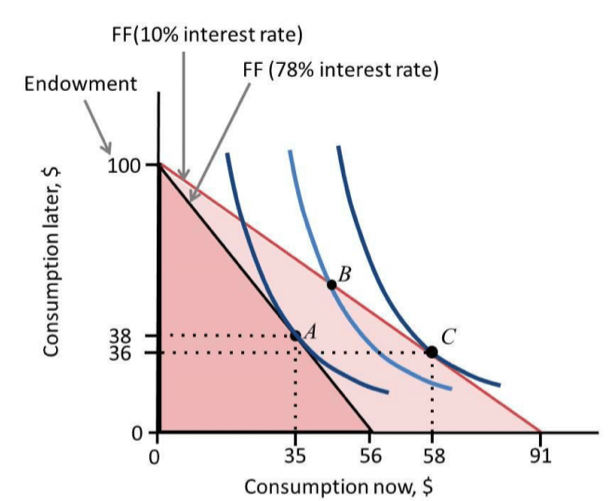
\includegraphics[width=\textwidth]{../QuestionBankImage/OUP-U10-Q8-01.png}

\answer{B}
\begin{tasks}(1)
    \task In scenario 1, Mary is better off choosing B than A.
        \details{B is not a feasible option under scenario 1.}
    \task The substitution and income effects of the interest rate fall work in the opposite directions for consumption in period 2.
        \details{The substitution effect would encourage Mary to consume less in period 2 (cheaper borrowing costs for period 1 consumption), while the income effect would encourage Mary to consume more in period 2.}
    \task The fall in the interest rate always results in a rise in consumption in both periods.
        \details{This is true for period 1 consumption, where substitution and income effects work in the same direction. For period 2 consumption, they work in opposite directions and may results in a fall in consumption if the substitution effect dominates the income effect (as depicted in this case).}
    \task Mary is more impatient at her optimal choice after the interest rate fall.
        \details{The marginal rate of substitution is lower at C than at A. Therefore she is less impatient after the rate fall.}
\end{tasks}


\Question (OUP-U10-Q15)
The diagram depicts Marco’s choice of consumptions in periods 1 and 2. He has \$100 worth of grain in period 1 and no income in period 2. Marco decides to consume \$65 worth of grain in period 1, sell the remaining grain and lend the money at an interest rate of 10\%, which he uses to buy grain for his consumption in period 2 (point A). Which of the following statements regarding his balance sheet is correct?

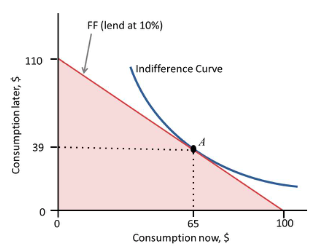
\includegraphics[width=\textwidth]{../QuestionBankImage/OUP-U10-Q15-01.png}

\answer{D}
\begin{tasks}(1)
    \task The asset after lending but before consumption is \$65.
        \details{Even when he has lent the money, the money remains on the balance sheet as an asset. Therefore the asset after lending but before consumption is \$100.}
    \task The asset after consumption in period 1 is \$39.
        \details{The asset after consumption in period 1 is the amount that Marco has saved, which is \$35.}
    \task The net worth before consumption in period 2 is \$0.
        \details{Marco’s assets in period 2 before consumption is \$39. He has no liabilities. Therefore his net worth is \$39.}
    \task Marco’s liabilities remain at 0 at all times.
        \details{In this scenario Marco does not borrow at all at any time. Therefore his liability remains 0 at all times.}
\end{tasks}




\Question (OUP-U10-Q20)
Which of the following statements is correct?
\answer{B}
\begin{tasks}(1)
    \task If the annually compounding interest rate is 5\%, then the present value of £100 in two years’ time is £90.91.
        \details{$PV = 100/(1+0.05)^2 = 90.70.$}
    \task If the annually compounding interest rate is 5\%, then the total present value (in Year 0) of receiving £100 at the end of Year 1 and £100 at the end of Year 2 is £185.94.
        \details{$PV = 100/(1 + 0.05) + 100/(1+0.05)^2 = 185.94.$}
    \task £95 today is worth the same as £100 in one year’s time if the interest rate is 5\%.
        \details{The present value of £100 in one year’s time at the interest rate of 5\% is $PV = 100/(1 + 0.05) = 95.24$. Therefore £95.24 today is worth the same as £100 in one year’s time.}
    \task If you pay £96 for an investment that pays £100 in one year’s time when the interest rate is 5\%, then your net present value is £0.76.
        \details{The present value of £100 in one year’s time at the interest rate of 5\% is $PV = 100/(1 + 0.05) = 95.24$. If C is the cost of the investment then the net present value is given by $NPV = PV - C$, which in this case is 95.24 - 96 = -£0.76, i.e. negative.}
\end{tasks}



\Question (OUP-U10-Q23)
The following is a simplified balance sheet of a commercial bank. Based on this information, which of the following statements is correct?
    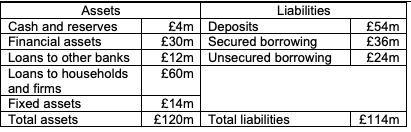
\includegraphics[width=\textwidth]{../QuestionBankImage/OUP-U10-Q23-01.png}

\answer{D}
\begin{tasks}(1)
    \task £34 million of the assets are owned by the bank.
        \details{The bank owns the cash and reserves, the financial assets, and the fixed assets. The loans are owned by the borrowers. Therefore 4 + 30 + 14 = £48 million of the assets are owned by the bank.}
    \task 	The value of the bank’s equity is £120 million.
        \details{The equity is the bank’s net worth, the value of which is 120 - 114 = £6 million.}
    \task The bank’s leverage ratio is 95.
        \details{That would be the leverage ratio normally defined for non-banks (total liabilities/total assets). For banks the leverage ratio is defined as total assets/net worth, which in this case is 120/6 = 20.}
    \task A fall of over 5\% in the asset value would make the bank insolvent.
        \details{The bank’s leverage is 120/6 = 20, meaning that the equity value is only 5\% of the total assets. This means that a fall of over 5\% in the asset value would wipe away its equity, making it insolvent.}
\end{tasks}



\Question (OUP-U10-Q12)
The diagram depicts Marco’s choice of consumptions in periods 1 and 2. He has \$100 worth of grain in period 1 and no income in period 2. Marco has two choices. In scheme 1, he can sell the grain that he does not consume and lend the money at 10\%. In scheme 2, he can invest the grain that he does not consume (e.g. planting as seed) for a return of 50\%. Which of the following statements is correct?
    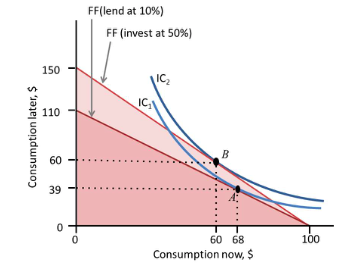
\includegraphics[width=\textwidth]{../QuestionBankImage/OUP-U10-Q12-01.png}
\answer{D}
\begin{tasks}(1)
    \task Marco is less impatient at B than at A.
        \details{The marginal rate of substitution is higher at B than at A. Therefore Marco is more impatient at B than at A.}
    \task Going from scheme 1 to scheme 2, the substitution and income effects have opposite effects on period 2 consumption.
        \details{A higher return means (i) it is more expensive to consume in period 1, and therefore the substitution effect is positive for period 2 consumption, and (ii) higher total income, which implies that the income effect is also positive for period 2 consumption.}
    \task Marco can do better than consumption choice B by investing all of his grain and consuming the output in period 2.
        \details{B is the point of tangency between the scheme 2 feasible frontier and the highest attainable indifference curve. Therefore he would be worse off at any other point on the feasible frontier, including at the ends.}
    \task Marco can do better than consumption choice B by investing all of his grain and borrowing against his period 2 output.
        \details{This shifts the feasible frontier out pivoted at the vertical axis, allowing Marco to attain higher indifference curves than $IC_2$.}
\end{tasks}



\Question (TEA-U10-Q2)
The following diagram depicts Julia’s choice of consumption now and consumption later (next period). She has no income now and an income of \$115 later. The current interest rate is 15\%. Based on this information, which of the following statements is correct?
    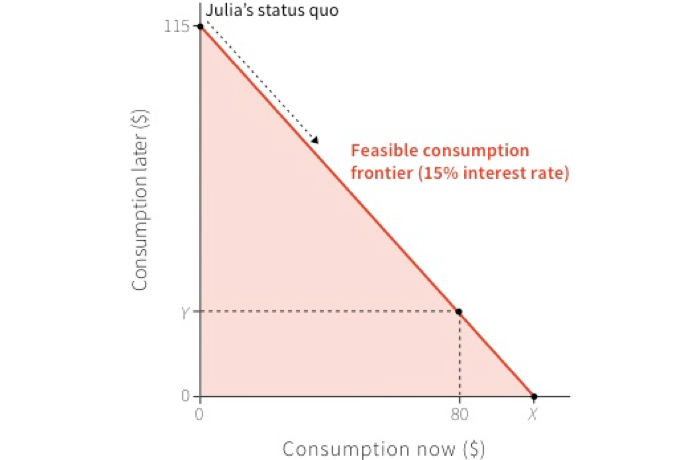
\includegraphics[width=\textwidth]{../QuestionBankImage/TEA-U10-Q2-01.png}
\answer{B}
\begin{tasks}(1)
    \task The maximum that Julia can borrow to spend now is \$91.
        \details{The maximum that Julia can borrow is $\$115/(1 + 0.15) = \$100$. This is the maximum that she can spend now.}
    \task If Julia borrows \$80 to spend now, she will have \$23 to spend later.
        \details{If Julia borrows \$80, she has to pay back $\$80 \times  1.15 = \$92$, so she will have \$115 - \$92 = \$23 to spend later.}
    \task The consumption choice of \$60 now and \$50 later is a feasible option.
        \details{When Julia borrows \$60, she has to pay back $\$60 \times  1.15 = \$69$, so she will have \$115 - \$69 = \$46 to spend later. Therefore the choice (60, 50) is not in her feasible set.}
    \task The feasible set will be smaller when the interest rate is 10\%.
        \details{When the interest rate falls, Julia’s feasible set will become larger: she will be able to borrow a maximum of \$115/(1 + 0.1) = \$104.5 to spend now.}
\end{tasks}



\Question (TEA-U10-Q5)
The diagram depicts Marco’s choice of consumptions now and later (next period). He has \$100 worth of grain now and no income later. Marco has two choices. In scheme 1, he can store the grain that he does not consume now. This results in a loss of 20\% of the grain due to pests and rotting. In scheme 2, he can sell the grain that he does not consume and lend the money at 10\%. Based on this information, which of the following statements is correct?
    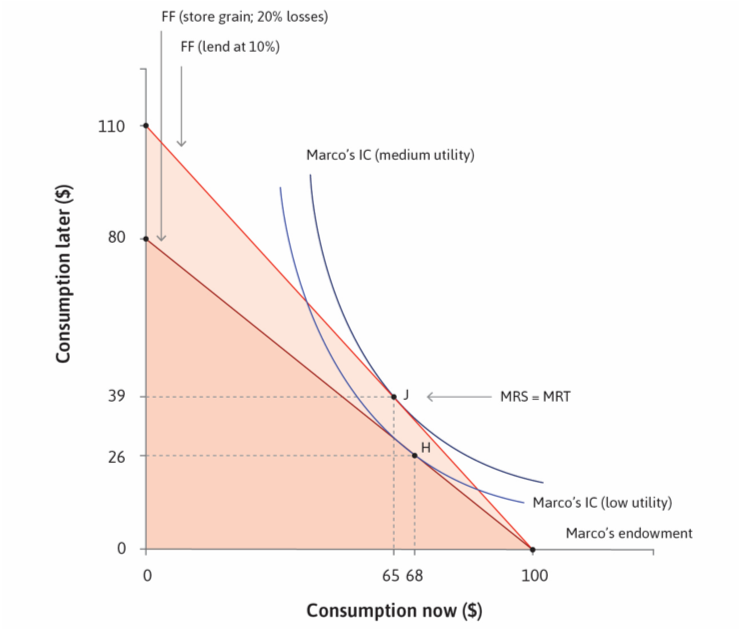
\includegraphics[width=\textwidth]{../QuestionBankImage/TEA-U10-Q5-01.png}
\answer{C}
\begin{tasks}(1)
    \task The substitution effect implies that Marco will consume more now under scheme 2 than under scheme 1.
        \details{The higher MRT in scheme 2 means that Marco will want to consume less now under scheme 2.}
    \task The income effect implies that Marco will consume more later and less now under scheme 2 than under scheme 1.
        \details{The income effect means that Marco will want to consume more in both periods (now and later) under scheme 2.}
    \task Marco will unambiguously consume more later under scheme 2 than in scheme 1.
        \details{The income and substitution effects work in the same direction, so Marco will consume more later under scheme 2.}
    \task Marco will unambiguously consume less now under scheme 2 than in scheme 1.
        \details{This depends on the relative size of the negative substitution effect and the positive income effect. If the latter more than offsets the former then Marco will also consume more now.}
\end{tasks}




\Question (UCL-S16-Q6)
The following diagram depicts Julia’s choice of consumption in periods 1 and 2. She has no income in period 1 and an income of \$115 in period 2. The current interest rate is 15\%. Based on this information, which of the following statements is correct?
    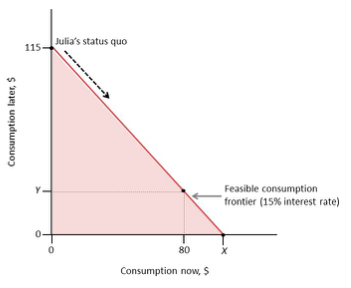
\includegraphics[width=\textwidth]{../QuestionBankImage/UCL-S16-Q6-01.png}
\answer{B}
\begin{tasks}(1)
    \task The maximum that Julia can borrow to spend in period 1 is \$91.
        \details{The maximum Julia can borrow to spend in period 1 is \$100 (= 115/1.15). She borrows \$100, she needs to pay back the principal and \$15 in interest, so in period 2 she will consume \$0 but she will have repaid her debt.}
    \task If Julia borrows \$80 to spend in period 1, she will have \$23 to spend in period 2.
        \details{If she borrows \$80, she is giving up \$80 in period 2, and she will need to pay \$12 in interest. Therefore, in period 2 she will only be able to consume \$115 - (\$80 + \$12) = \$23.}
    \task The consumption choice of \$60 in period 1 and \$50 in period 2 is a feasible option.
        \details{If she borrows \$60, she will need to repay the principal and \$9 in interest. So in period 2 she will only be able to consume at most \$115 - (\$60 + \$9) = \$46. She cannot consume \$50 in period 2.}
\end{tasks}



\Question (UCL-S17-Q13)
Which of the following statements about liquidity and solvency is/are true?
\answer{A}
\begin{tasks}(1)
    \task The relevant items on the balance sheet to assess solvency are total liabilities and total assets.
        \details{Solvency is defined as the value of assets exceeding the value of liabilities, so we need total assets and liabilities in order to assess solvency.}
    \task Allowing banks to borrow from the central bank at a penalty rate of interest can deal with a bank’s solvency but not liquidity problem.
        \details{Borrowing increases a bank's liabilities, so the converse is true: Allowing banks to borrow from the central bank at a penalty rate of interest can deal with a bank’s liquidity but not solvency problem.}
    \task If a bank admits that many of its loans are ‘non-performing’ and unlikely to be repaid, this increases its liabilities.
        \details{Bank loans are on the asset side of its balance sheet, so declaring loans as 'non-performing' increases its assets.}
\end{tasks}

\end{Exercise}

\end{document}
